% ----------------------------------------------------------
% Classificação dos Gargalos
% ----------------------------------------------------------
\chapter{Classificação dos Gargalos}
\label{cap:classificacao}
% ----------------------------------------------------------

Este capítulo descreve a implementação prática do classificador determinístico heurístico de gargalos corporativos e a parametrização do modelo não-supervisionado de aprendizado de máquina \textit{K-Means}. Apresentam-se os critérios físicos adotados para a árvore de decisão, as variáveis selecionadas para a modelagem dos clusters de Access Points e a discussão empírica consolidada dos resultados gerados pelo pipeline de dados.

\section{Classificação de Gargalos Baseada em Limiares}
\label{sec:classificacao_limiares_cap}

A identificação automática das causas de degradação de vazão em cada AP foi modelada inicialmente por meio de uma árvore de decisão com limiares físicos heurísticos baseados em boas práticas de gerência de redes corporativas. Esse classificador determinístico rotula o estado operacional de cada amostra de telemetria em um de cinco perfis de gargalos físicos e de infraestrutura, além do estado ideal:

\begin{enumerate}
	\item \textbf{Baixa Qualidade de Enlace (Gargalo G1)}: Ocorre quando a potência média de recepção do rádio é atenuada. Define-se o limiar de gatilho para amostras em que o sinal físico recebido pelo AP (\textit{signal}) é estritamente inferior a $-75$~dBm;
	\item \textbf{Congestionamento do Meio (Gargalo G2)}: Caracteriza o esgotamento de recursos decorrente da densidade de dispositivos. É disparado quando o número de clientes ativos simultâneos conectados no mesmo AP e minuto é maior ou igual a $15$ dispositivos;
	\item \textbf{Interferência ou SNR Ruim (Gargalo G3)}: Identifica a perda de integridade física dos quadros de rádio decorrente de interferência externa. É ativado quando o ruído de fundo (\textit{noise}) é superior a $-90$~dBm, ou quando a relação sinal-ruído (\textit{Signal-to-Noise Ratio} -- SNR) é inferior a $20$~dB em clientes que possuem boa intensidade de sinal recebido (maior ou igual a $-75$~dBm);
	\item \textbf{Instabilidade de Roaming (Gargalo G4)}: Mapeia o comportamento de instabilidade na associação de clientes. É disparado para dispositivos clientes que registraram mais de $5$ transições rápidas de AP (\textit{roaming}) no período de observação de um dia;
	\item \textbf{Gargalo de Infraestrutura Cabeada (Gargalo G5)}: Identifica a saturação do enlace físico que conecta o AP ao \textit{switch} de acesso da rede local. É acionado quando a taxa de throughput agregada sustentada no rádio atinge ou supera o patamar de $90$~Mbps, aproximando-se do limite de vazão útil de uma porta física \textit{Fast Ethernet} de $100$~Mbps;
	\item \textbf{Operação Ideal (Sem Gargalos)}: Amostras que apresentam sinal físico saudável (maior ou igual a $-75$~dBm), ausência de congestionamento de canal ou interferência eletromagnética crônica, sem ocorrência de instabilidade de associação ou saturação de cabeamento.
\end{enumerate}

Essa divisão sistemática permite que os administradores identifiquem se a degradação de sinal de um setor decorre de barreiras estruturais da edificação (G1), subdimensionamento do número de rádios instalados (G2), poluição do espectro local por canais concorrentes (G3), instabilidade de antena do cliente (G4) ou obsolescência dos equipamentos de rede cabeada e switches locais (G5).

\section{Agrupamento Operacional de Access Points (K-Means)}
\label{sec:kmeans_desenvolvimento_cap}

Com o objetivo de validar a classificação de gargalos e definir o comportamento operacional típico de cada rádio de forma automatizada e livre de vieses heurísticos manuais, aplicou-se o algoritmo de aprendizado de máquina não-supervisionado \textit{K-Means}. 

O algoritmo foi parametrizado para identificar exatamente $K=4$ clusters operacionais para cada fabricante. As variáveis de entrada selecionadas para caracterizar o espaço métrico multidimensional de operação de cada rádio $j$ foram calculadas a partir das médias temporais consolidadas:

\begin{equation}
\label{eq:features_kmeans_cap}
X_j = \{ C_j, T_j, S_j, R_j \}
\end{equation}

onde:
\begin{itemize}
	\item $C_j$ representa a média de dispositivos clientes conectados simultaneamente ao rádio $j$;
	\item $T_j$ representa a média de vazão agregada (\textit{throughput}) do rádio $j$, mensurada em Mbps;
	\item $S_j$ representa a média de potência de sinal físico recebido (\textit{signal}) no rádio $j$, medida em dBm;
	\item $R_j$ representa a média da taxa de retransmissão de quadros de dados físicos no rádio $j$, expressa em percentual.
\end{itemize}

Antes de aplicar a clusterização, realizou-se a normalização z-score das variáveis de entrada por meio do módulo \textit{StandardScaler}. Esse passo metodológico é essencial em algoritmos de distância euclidiana como o \textit{K-Means}, pois impede que métricas com escalas numéricas superiores (como as amostras físicas em dBm ou volumes agregados) dominem o cálculo de distância em relação a métricas com intervalos menores (como número médio de usuários).

A normalização z-score para uma variável $x$ é dada pela Equação~\ref{eq:zscore_cap}:

\begin{equation}
\label{eq:zscore_cap}
z = \frac{x - \mu}{\sigma}
\end{equation}

onde $\mu$ representa a média amostral e $\sigma$ o desvio padrão da respectiva métrica.

A execução do modelo de agrupamento classifica cada rádio no cluster com a menor distância quadrada média até o centróide representante, originando os perfis descritos como Grupo A (Muito Carregado), Grupo B (Pouco Utilizado), Grupo C (Carga Moderada) e Grupo D (Baixa Qualidade de Sinal / Instável).

\section{Resultados da Classificação e do Agrupamento}
\label{sec:resultados_classificacao_cap}

Abaixo são detalhados e discutidos os resultados práticos gerados na classificação de telemetria e no agrupamento não-supervisionado de pontos de acesso.

\section{Classificação de Gargalos de Rede}

\subsection{Limiares de Decisão Estabelecidos}

\begin{enumerate}
  \item \textbf{G1: Baixa Qualidade de Enlace}: Potência física de sinal recebido pelo AP (\texttt{signal}) < \texttt{-75 dBm}.
  \item \textbf{G2: Congestionamento do Meio}: Número de clientes simultâneos conectados no mesmo AP e minuto >= 15.
  \item \textbf{G3: Interferência / SNR Ruim}: Ruído de fundo (\texttt{noise}) > \texttt{-90 dBm} ou SNR < \texttt{20 dB} em clientes com bom sinal (>= -75 dBm).
  \item \textbf{G4: Instabilidade de Roaming}: Clientes (MAC) que registraram > 5 trocas de AP no período de observação.
  \item \textbf{G5: Gargalo Cabeado (FE)}: Throughput de tráfego agregado sustentado do AP >= 90 Mbps (limite de interface Fast Ethernet de 100 Mbps).


\end{enumerate}
\subsection{Tabela Geral de Ocorrência e Impacto de Gargalos}

A Tabela Geral de Ocorrência apresenta as taxas e consequências físicas associadas a cada tipo de gargalo detectado de forma isolada ao longo do monitoramento de produção.

\begin{table}[H]
\IBGEtab{%
  \caption{Tabela Geral de Ocorrência e Impacto de Gargalos}%
  \label{tab:data_classificacao_gargalos_1}%
}{%
  \centering\footnotesize
  \resizebox{0.92\textwidth}{!}{%
    \begin{tabular}{lccccc}
      Fabricante & Categoria de Gargalo & Amostras (N) & Porcentagem (\%) & Throughput Cliente (Méd/Med) [Mbps] & Retransmissões (Méd/Med) [\%] \\
      \midrule
      \textbf{Ruckus} & G1: Baixa Qualidade de Enlace & 192.148 & 43,08\% & 0,502 / 0,129 & 5,37\% / 0,00\% \\
      \textbf{UniFi} & G1: Baixa Qualidade de Enlace & 13.663 & 26,29\% & 0,030 / 0,000 & 35,27\% / 25,00\% \\
      \textbf{Ruckus} & G2: Congestionamento do Meio & 198.696 & 44,54\% & 0,484 / 0,125 & 4,73\% / 0,00\% \\
      \textbf{UniFi} & G2: Congestionamento do Meio & 1.344 & 2,59\% & 0,227 / 0,002 & 22,50\% / 14,40\% \\
      \textbf{Ruckus} & G3: Interferência / SNR Ruim & 0 & 0,00\% & 0,000 / 0,000 & 0,00\% / 0,00\% \\
      \textbf{UniFi} & G3: Interferência / SNR Ruim & 544 & 1,05\% & 0,101 / 0,000 & 32,45\% / 30,90\% \\
      \textbf{Ruckus} & G4: Instabilidade de Roaming & 262.678 & 58,89\% & 0,397 / 0,109 & 6,39\% / 0,00\% \\
      \textbf{UniFi} & G4: Instabilidade de Roaming & 12.630 & 24,30\% & 0,180 / 0,000 & 17,10\% / 10,00\% \\
      \textbf{Ruckus} & G5: Gargalo Cabeado (FE) & 33 & 0,01\% & 6,219 / 0,144 & 2,11\% / 0,75\% \\
      \textbf{UniFi} & G5: Gargalo Cabeado (FE) & 0 & 0,00\% & 0,000 / 0,000 & 0,00\% / 0,00\% \\
      \textbf{Ruckus} & Sem Gargalos & 58.454 & 13,10\% & 0,493 / 0,100 & 4,49\% / 0,00\% \\
      \textbf{UniFi} & Sem Gargalos & 27.115 & 52,17\% & 0,384 / 0,001 & 17,39\% / 9,30\% \\
      \bottomrule
    \end{tabular}%
  }%
}{%
  \fonte{Produzido pelos autores.}%
}
\end{table}


\subsection{Análise de Desempenho e Carga por Access Point}

Abaixo são apresentados os perfis consolidados de carga e desempenho de cada Access Point mapeado na coleta, ordenados pelo throughput agregado médio (indicador de demanda atendida).

\subsubsection{Rede Ruckus (APs MAC Simplificados)}

\begin{table}[H]
\IBGEtab{%
  \caption{Rede Ruckus (APs MAC Simplificados)}%
  \label{tab:data_classificacao_gargalos_2}%
}{%
  \centering\footnotesize
  \resizebox{\textwidth}{!}{%
    \begin{tabular}{lcccccccc}
      Access Point & Amostras (N) & Clientes Médios (Pico) & Throughput Agregado Médio (Max) [Mbps] & Sinal Médio [dBm] & Retransmissões Médias [\%] & Throughput Médio p/ Cliente [Mbps] & Equidade Média (Jain) & Perfil Operacional (Cluster) \\
      \midrule
      \textbf{RK-fea0} & 38.146 & 22,7 (max 64) & 15,397 (max 111,108) & -75,7 & 3,75\% & 0,638 & 0,2935 & Grupo A: Muito Carregado \\
      \textbf{RK-0d40} & 35.809 & 20,6 (max 49) & 11,105 (max 54,074) & -75,6 & 4,05\% & 0,538 & 0,3067 & Grupo A: Muito Carregado \\
      \textbf{RK-2fd0} & 25.176 & 16,4 (max 42) & 8,284 (max 46,102) & -74,2 & 4,17\% & 0,520 & 0,3495 & Grupo C: Carga Moderada \\
      \textbf{RK-27d0} & 42.244 & 21,4 (max 55) & 8,205 (max 37,443) & -75,7 & 6,61\% & 0,390 & 0,3261 & Grupo C: Carga Moderada \\
      \textbf{RK-35c0} & 23.807 & 13,9 (max 36) & 8,074 (max 57,785) & -74,1 & 7,44\% & 0,565 & 0,3613 & Grupo C: Carga Moderada \\
      \textbf{RK-4050} & 29.173 & 17,1 (max 46) & 8,044 (max 32,117) & -72,5 & 5,27\% & 0,467 & 0,3457 & Grupo C: Carga Moderada \\
      \textbf{RK-efe0} & 30.711 & 14,0 (max 46) & 7,051 (max 56,451) & -65,9 & 4,39\% & 0,554 & 0,3868 & Grupo C: Carga Moderada \\
      \textbf{RK-51f0} & 38.558 & 17,3 (max 41) & 6,383 (max 47,167) & -74,7 & 5,98\% & 0,373 & 0,3636 & Grupo C: Carga Moderada \\
      \textbf{RK-9660} & 19.921 & 13,2 (max 35) & 5,786 (max 53,827) & -73,9 & 4,95\% & 0,456 & 0,3653 & Grupo C: Carga Moderada \\
      \textbf{RK-1e40} & 12.794 & 11,9 (max 39) & 5,416 (max 84,886) & -74,2 & 6,05\% & 0,458 & 0,4185 & Grupo C: Carga Moderada \\
      \textbf{RK-3180} & 20.228 & 13,1 (max 35) & 5,264 (max 53,483) & -74,6 & 3,92\% & 0,400 & 0,3985 & Grupo C: Carga Moderada \\
      \textbf{RK-1060} & 15.381 & 9,9 (max 26) & 4,367 (max 44,399) & -75,0 & 3,97\% & 0,457 & 0,3878 & Grupo C: Carga Moderada \\
      \textbf{RK-0780} & 1.483 & 15,7 (max 29) & 3,805 (max 17,069) & -69,5 & 4,04\% & 0,236 & 0,3267 & Grupo C: Carga Moderada \\
      \textbf{RK-42a0} & 11.694 & 7,4 (max 28) & 3,737 (max 34,312) & -70,8 & 4,36\% & 0,497 & 0,4808 & Grupo B: Pouco Utilizado \\
      \textbf{RK-7090} & 12.790 & 8,3 (max 25) & 3,667 (max 28,851) & -73,4 & 7,15\% & 0,413 & 0,4018 & Grupo B: Pouco Utilizado \\
      \textbf{RK-e8a0} & 15.959 & 10,5 (max 31) & 3,541 (max 61,206) & -72,4 & 5,35\% & 0,405 & 0,4056 & Grupo B: Pouco Utilizado \\
      \textbf{RK-1730} & 21.933 & 9,0 (max 26) & 3,479 (max 29,586) & -74,3 & 7,85\% & 0,465 & 0,4211 & Grupo D: Baixa Qualidade de Sinal \\
      \textbf{RK-3b10} & 7.700 & 6,9 (max 17) & 2,821 (max 40,003) & -72,7 & 5,77\% & 0,408 & 0,4933 & Grupo B: Pouco Utilizado \\
      \textbf{RK-1c10} & 9.343 & 6,5 (max 22) & 2,810 (max 31,876) & -75,0 & 9,32\% & 0,421 & 0,4769 & Grupo D: Baixa Qualidade de Sinal \\
      \textbf{RK-f3f0} & 9.861 & 4,1 (max 13) & 2,169 (max 47,419) & -71,2 & 7,16\% & 0,504 & 0,4853 & Grupo B: Pouco Utilizado \\
      \textbf{RK-5fe0} & 6.723 & 4,4 (max 12) & 1,977 (max 55,447) & -72,3 & 8,25\% & 0,422 & 0,5014 & Grupo B: Pouco Utilizado \\
      \textbf{RK-3440} & 11.513 & 8,9 (max 34) & 1,942 (max 26,487) & -77,0 & 11,41\% & 0,228 & 0,4037 & Grupo D: Baixa Qualidade de Sinal \\
      \textbf{RK-edd0} & 1.855 & 3,4 (max 8) & 1,807 (max 8,914) & -73,7 & 1,95\% & 0,567 & 0,5890 & Grupo B: Pouco Utilizado \\
      \textbf{RK-dcd0} & 3.258 & 4,7 (max 16) & 1,044 (max 8,827) & -74,7 & 7,27\% & 0,231 & 0,4471 & Grupo D: Baixa Qualidade de Sinal \\
      \bottomrule
    \end{tabular}%
  }%
}{%
  \fonte{Produzido pelos autores.}%
}
\end{table}

\subsubsection{Rede UniFi (APs Cadastrados)}

\begin{table}[H]
\IBGEtab{%
  \caption{Rede UniFi (APs Cadastrados)}%
  \label{tab:data_classificacao_gargalos_3}%
}{%
  \centering\footnotesize
  \resizebox{\textwidth}{!}{%
    \begin{tabular}{lcccccccc}
      Access Point & Amostras (N) & Clientes Médios (Pico) & Throughput Agregado Médio (Max) [Mbps] & Sinal Médio [dBm] & Retransmissões Médias [\%] & Throughput Médio p/ Cliente [Mbps] & Equidade Média (Jain) & Perfil Operacional (Cluster) \\
      \midrule
      \textbf{Lab Redes} & 8.894 & 7,7 (max 21) & 2,078 (max 44,247) & -67,0 & 23,29\% & 0,224 & 0,2861 & Grupo A: Muito Carregado \\
      \textbf{Guarita Entrada} & 9.280 & 4,8 (max 19) & 1,708 (max 14,370) & -68,0 & 32,74\% & 0,452 & 0,3175 & Grupo A: Muito Carregado \\
      \textbf{B-301\_D} & 1.426 & 2,8 (max 10) & 1,636 (max 34,411) & -63,8 & 14,41\% & 0,448 & 0,4291 & Grupo D: Baixa Retransmissão / Estável \\
      \textbf{Lab Expressao} & 3.629 & 6,5 (max 17) & 1,246 (max 13,302) & -63,1 & 19,37\% & 0,166 & 0,3221 & Grupo A: Muito Carregado \\
      \textbf{B-300\_E} & 1.706 & 2,8 (max 11) & 0,923 (max 35,659) & -67,1 & 12,42\% & 0,370 & 0,4370 & Grupo D: Baixa Retransmissão / Estável \\
      \textbf{B-100\_Recepcao} & 2.756 & 2,5 (max 9) & 0,848 (max 40,739) & -65,3 & 13,27\% & 0,252 & 0,4495 & Grupo D: Baixa Retransmissão / Estável \\
      \textbf{A-201} & 2.676 & 2,2 (max 7) & 0,738 (max 15,183) & -65,3 & 17,58\% & 0,344 & 0,5029 & Grupo D: Baixa Retransmissão / Estável \\
      \textbf{C-304 Rack} & 2.840 & 3,1 (max 11) & 0,726 (max 34,293) & -65,6 & 18,13\% & 0,247 & 0,4487 & Grupo D: Baixa Retransmissão / Estável \\
      \textbf{A400-1} & 3.595 & 2,5 (max 9) & 0,621 (max 16,116) & -67,9 & 19,18\% & 0,194 & 0,4575 & Grupo D: Baixa Retransmissão / Estável \\
      \textbf{A400-Rack} & 1.595 & 2,1 (max 6) & 0,616 (max 36,024) & -65,5 & 14,75\% & 0,271 & 0,5202 & Grupo D: Baixa Retransmissão / Estável \\
      \textbf{B-200\_Bibliotecaria} & 2.436 & 2,6 (max 7) & 0,478 (max 22,187) & -61,7 & 16,06\% & 0,211 & 0,4695 & Grupo D: Baixa Retransmissão / Estável \\
      \textbf{B-200\_D} & 441 & 1,7 (max 4) & 0,380 (max 22,112) & -70,4 & 15,77\% & 0,340 & 0,5653 & Grupo D: Baixa Retransmissão / Estável \\
      \textbf{A100-recepçao} & 2.184 & 1,7 (max 5) & 0,377 (max 8,115) & -68,9 & 15,13\% & 0,198 & 0,5594 & Grupo D: Baixa Retransmissão / Estável \\
      \textbf{B-100\_Empresa\_Junior} & 265 & 1,7 (max 4) & 0,313 (max 5,991) & -68,9 & 28,11\% & 0,181 & 0,5553 & Grupo B: Pouco Utilizado \\
      \textbf{A101-Novo} & 4.787 & 2,4 (max 7) & 0,222 (max 16,515) & -66,9 & 20,74\% & 0,091 & 0,4859 & Grupo B: Pouco Utilizado \\
      \textbf{PICO-H-100} & 1.144 & 1,5 (max 6) & 0,207 (max 8,336) & -46,1 & 35,49\% & 0,097 & 0,5129 & Grupo C: Alta Retransmissão \\
      \textbf{Biblioteca-2} & 1.729 & 2,0 (max 8) & 0,167 (max 8,738) & -74,1 & 19,55\% & 0,074 & 0,5107 & Grupo B: Pouco Utilizado \\
      \textbf{Pico-D200} & 350 & 1,2 (max 3) & 0,084 (max 4,730) & -65,8 & 28,57\% & 0,073 & 0,7003 & Grupo B: Pouco Utilizado \\
      \textbf{PICOH-206} & 241 & 1,1 (max 2) & 0,044 (max 1,868) & -66,7 & 19,25\% & 0,043 & 0,6380 & Grupo B: Pouco Utilizado \\
      \bottomrule
    \end{tabular}%
  }%
}{%
  \fonte{Produzido pelos autores.}%
}
\end{table}


\subsection{Análise de Distribuição e Frequência}

O histograma geral ilustra as taxas percentuais de ocorrência de cada tipo de gargalo. Os resultados sugerem disparidades sistemáticas entre as marcas decorrentes do posicionamento físico dos APs e da ocupação do campus.

\begin{enumerate}
  \item \textbf{Baixa Qualidade de Enlace (G1)}:
  \begin{itemize}
    \item Afeta \textbf{43,08\%} das amostras na Ruckus e \textbf{26,29\%} na UniFi. Esse perfil elevado indica que uma porção considerável dos usuários se posicionou nas bordas de cobertura ou em zonas de sombra de sinal Wi-Fi nas dependências do campus.
\end{itemize}
  \item \textbf{Congestionamento do Meio (G2)}:
  \begin{itemize}
    \item A Ruckus registrou \textbf{44,54\%} de suas amostras sob congestionamento (APs com 15 ou mais clientes simultâneos), enquanto a UniFi teve apenas \textbf{2,59\%} sob essa condição. Essa discrepância é consistente com o fato de a rede Ruckus atender a setores de maior fluxo de estudantes, suportando forte densidade.
\end{itemize}
  \item \textbf{Interferência (G3)}:
  \begin{itemize}
    \item Este gargalo teve incidência nula na Ruckus (\textbf{0,00\%}) e ínfima na UniFi (\textbf{1,05\%}) sob os critérios rigorosos avaliados de forma isolada, sugerindo que os cenários de alta retransmissão estão fundamentalmente vinculados à fraca qualidade de sinal ou ao excessivo congestionamento e trocas de AP.
\end{itemize}
  \item \textbf{Instabilidade de Roaming (G4)}:
  \begin{itemize}
    \item Afetou massivos \textbf{58,89\%} dos registros de Ruckus e \textbf{24,30\%} de UniFi. Dispositivos móveis realizam abundantes transições ou persistem conectados a APs distantes (\textit{sticky clients}), evidenciando o gargalo mais disseminado da infraestrutura corporativa do campus.
\end{itemize}
  \item \textbf{Limitação de Infraestrutura Cabeada (G5)}:
  \begin{itemize}
    \item Virtualmente nula (\textbf{0,01\%} na Ruckus e \textbf{0,00\%} na UniFi). O tráfego não saturou de forma crônica as portas Fast Ethernet, indicando que o gargalo de \textit{backhaul} cabeado não é a atual limitação de desempenho.


\end{itemize}
\end{enumerate}
\subsection{Análise de Consequências e Hipóteses}

\subsubsection{Impacto no Throughput}

\begin{itemize}
  \item \textbf{Padrão de Throughput (Sem Gargalos)}: Sob condições ideais ("Sem Gargalos"), o throughput médio por cliente foi de \texttt{0.493 Mbps} no Ruckus e \texttt{0.384 Mbps} no UniFi.
  \item \textbf{Consequência de Baixa Qualidade de Sinal (G1)}: No Ruckus, a vazão média manteve-se em \texttt{0.502 Mbps} (redução de -2,0\% em relação ao ideal). Já na UniFi, a vazão despencou para \texttt{0.030 Mbps} (redução severa de 92,1\%), sugerindo o alto impacto da atenuação física sobre o desempenho prático dos clientes.
  \item \textbf{Consequência de Congestionamento (G2)}: A vazão média manteve-se em \texttt{0.484 Mbps} no Ruckus e registrou queda na UniFi para \texttt{0.227 Mbps} (redução de 40,9\% em relação à condição ideal), refletindo o efeito do compartilhamento de tempo de transmissão aérea (CSMA/CA).
  \item \textbf{Consequência de Interferência (G3)}: Não houve registros isolados suficientes no Ruckus (incidência de 0,00\%), enquanto a UniFi registrou queda significativa da vazão média para \texttt{0.101 Mbps} (redução de 73,7\% em relação ao ideal).
  \item \textbf{Consequência de Instabilidade de Roaming (G4)}: O throughput médio de clientes afetados por roaming frequente foi de \texttt{0.397 Mbps} no Ruckus (queda de 19,3\% em relação ao ideal) e \texttt{0.180 Mbps} no UniFi.

\end{itemize}
\subsubsection{Impacto nas Retransmissões}

\begin{itemize}
  \item \textbf{Padrão Esperado (Sem Gargalos)}: Sob condições ideais, as taxas médias de retransmissão situaram-se em \texttt{4.49\%} na Ruckus e \texttt{17.39\%} na UniFi.
  \item \textbf{Consequência de Baixa Qualidade de Sinal (G1)}: Sob sinal fraco, a taxa de retransmissão no Ruckus subiu levemente para \texttt{5.37\%} (aumento de 19,7\% em relação ao ideal). Na UniFi, contudo, observou-se a maior elevação registrada, alcançando \texttt{35.27\%} (um aumento de 102,8\% em relação ao ideal), indicando a degradação da integridade de quadros em enlaces atenuados.
  \item \textbf{Consequência de Congestionamento (G2)}: A taxa de retransmissão manteve-se estável na Ruckus (\texttt{4.73\%}) e na UniFi (\texttt{22.50\%}), sugerindo que a concorrência pelo meio não foi a causa primária para o aumento direto de retransmissões.
  \item \textbf{Consequência de Interferência (G3)}: Sem registros isolados na Ruckus, a UniFi registrou taxa de retransmissão elevada em \texttt{32.45\%} (aumento de 86,6\% em relação ao ideal), o que evidencia a ocorrência de colisões provocadas por ruído de RF.
  \item \textbf{Consequência de Instabilidade de Roaming (G4)}: A taxa no Ruckus variou ligeiramente para \texttt{6.39\%} (aumento de 42,4\% em relação ao ideal), enquanto a UniFi registrou taxa média de \texttt{17.10\%}.


\end{itemize}
\subsection{Clusterização e Perfil Operacional dos Access Points (K-Means)}

Para agrupar os Access Points com comportamentos operacionais semelhantes e gerar um mapa de diagnóstico útil, aplicou-se o algoritmo de aprendizado de máquina \textbf{K-Means} (com $K=4$ clusters para cada fabricante). A clusterização baseou-se na aplicação do algoritmo com normalização prévia das variáveis por meio do \texttt{StandardScaler} para evitar que a diferença de escalas (como potência de sinal em dBm vs clientes em unidades) distorcesse as distâncias euclidianas. 

A escolha do número de clusters ($K=4$) foi fundamentada por uma análise quantitativa cruzada baseada no Método do Cotovelo (inércia intra-cluster), no Índice de Silhueta (\textit{Silhouette Score}) e no Índice de Davies-Bouldin:
\begin{itemize}
  \item \textbf{Ambiente Ruckus}: A análise matemática revelou que o valor ótimo de partição é estritamente $K=4$. O índice de silhueta obteve seu pico máximo de \textbf{0,3383} em $K=4$ (comparado a 0,3157 para $K=2$, 0,3136 para $K=3$ e 0,3114 para $K=5$), enquanto o índice de Davies-Bouldin obteve o menor valor registrado de \textbf{0,7953} (contra 1,0517 em $K=2$ e 0,9440 em $K=3$), justificando matematicamente a divisão natural em quatro perfis operacionais de rádio;
  \item \textbf{Ambiente UniFi}: O Método do Cotovelo indicou uma redução acentuada da inércia de \textbf{45,27} ($K=2$) para \textbf{17,36} ($K=3$) e \textbf{11,13} ($K=4$), estabilizando-se em \textbf{8,89} para $K=5$. Embora as métricas de partição silhueta e Davies-Bouldin apontem que a rede UniFi divide-se fortemente em duas grandes macro-regiões ($K=2$, com silhueta de 0,5538 e Davies-Bouldin de 0,2959) devido à ociosidade crônica do espectro de 2,4 GHz, a adoção de $K=4$ foi mantida por simetria de modelo de análise comparativa. Esta escolha permitiu expor perfis operacionais minoritários de suma importância para o diagnóstico da rede, como o cluster de anomalia de RF (Grupo C: Alta Retransmissão).

\end{itemize}
As variáveis utilizadas para a clusterização foram: média de clientes, throughput agregado médio do AP, sinal físico médio e taxa média de retransmissões. Os centróides e perfis detalhados resultantes de cada cluster são discutidos a seguir:

\subsubsection{Perfis de Rádios Ruckus}

\begin{table}[H]
\IBGEtab{%
  \caption{Perfis de Rádios Ruckus}%
  \label{tab:data_classificacao_gargalos_4}%
}{%
  \centering\footnotesize
  \resizebox{0.92\textwidth}{!}{%
    \begin{tabular}{lcccc}
      Perfil Operacional (Cluster) & Média Clientes & Throughput Agregado Médio [Mbps] & Sinal Médio [dBm] & Retransmissões Médias [\%] \\
      \midrule
      \textbf{Grupo A: Muito Carregado} & 21,66 & 13,251 & -75,7 & 3,90\% \\
      \textbf{Grupo B: Pouco Utilizado} & 6,44 & 2,817 & -72,3 & 5,71\% \\
      \textbf{Grupo C: Carga Moderada} & 14,90 & 6,425 & -73,1 & 5,16\% \\
      \textbf{Grupo D: Baixa Qualidade de Sinal} & 7,25 & 2,319 & -75,3 & 8,96\% \\
      \bottomrule
    \end{tabular}%
  }%
}{%
  \fonte{Produzido pelos autores.}%
}
\end{table}

\begin{itemize}
  \item \textbf{Grupo A: Muito Carregado}: Representa os access points que operam sob intensa demanda de usuários (como \texttt{RK-fea0} e \texttt{RK-0d40}, com média de \texttt{21.66} clientes conectados e pico de tráfego agregado médio de \texttt{13.251 Mbps}). Apesar de operar sob alta concorrência de canal e sinal físico médio atenuado de \texttt{-75.7 dBm} (Gargalo G2), este grupo apresenta a menor taxa de retransmissão de toda a rede Ruckus (média de \texttt{3.90\%}). Este comportamento sugere o desempenho eficiente das tecnologias dinâmicas de filtragem espacial da Ruckus. A ação prática sugerida para estes APs visa aliviar a contenção de tempo aéreo (\textit{airtime}) por meio da ativação do direcionamento de banda (\textit{Band Steering}) e regras de balanceamento de carga ativo nas controladoras (Seção 6,2).
  \item \textbf{Grupo B: Pouco Utilizado}: Constituído por APs com baixo volume de tráfego (média de \texttt{2.817 Mbps}) e baixa concorrência (média de \texttt{6.44} clientes). O sinal físico médio é excelente (média de \texttt{-72.3 dBm}) e as retransmissões mantêm-se estáveis em \texttt{5.71\%}, representando pontos de ociosidade operacional na rede corporativa.
  \item \textbf{Grupo C: Carga Moderada}: Representa o perfil operacional típico nominal de RF da rede no campus (como os APs \texttt{RK-4050} e \texttt{RK-51f0}, com média de \texttt{14.90} clientes e throughput agregado médio de \texttt{6.425 Mbps}). Apresenta sinal médio de \texttt{-73.1 dBm} e taxa de retransmissão saudável de \texttt{5.16\%}.
  \item \textbf{Grupo D: Baixa Qualidade de Sinal}: Caracteriza os rádios severamente limitados pela qualidade física de recepção de sinal (como o AP \texttt{RK-3440} e \texttt{RK-dcd0}, com sinal médio degradado de \texttt{-75.3 dBm}). O baixo tráfego agregado registrado (\texttt{2.319 Mbps}) é consequência direta da elevada taxa de retransmissão de quadros (\texttt{8.96\%}), caracterizando o Gargalo G1. A ação recomendada para resolver este problema envolve o reposicionamento físico do AP para remover barreiras de atenuação e redimensionar a cobertura de rádio local (Seção 6,1).

\end{itemize}
\subsubsection{Perfis de Rádios UniFi}

\begin{table}[H]
\IBGEtab{%
  \caption{Perfis de Rádios UniFi}%
  \label{tab:data_classificacao_gargalos_5}%
}{%
  \centering\footnotesize
  \resizebox{0.92\textwidth}{!}{%
    \begin{tabular}{lcccc}
      Perfil Operacional (Cluster) & Média Clientes & Throughput Agregado Médio [Mbps] & Sinal Médio [dBm] & Retransmissões Médias [\%] \\
      \midrule
      \textbf{Grupo A: Muito Carregado} & 6,35 & 1,678 & -66,1 & 25,13\% \\
      \textbf{Grupo B: Pouco Utilizado} & 1,67 & 0,166 & -68,5 & 23,24\% \\
      \textbf{Grupo C: Alta Retransmissão} & 1,53 & 0,207 & -46,1 & 35,49\% \\
      \textbf{Grupo D: Baixa Retransmissão / Estável} & 2,41 & 0,734 & -66,2 & 15,67\% \\
      \bottomrule
    \end{tabular}%
  }%
}{%
  \fonte{Produzido pelos autores.}%
}
\end{table}

\begin{itemize}
  \item \textbf{Grupo A: Muito Carregado}: Engloba os APs da rede UniFi com maior atividade relativa (como \texttt{Lab Redes} e \texttt{Guarita Entrada}, com média de \texttt{6.35} clientes e throughput agregado médio de \texttt{1.678 Mbps}). O sinal médio é saudável (\texttt{-66.1 dBm}), mas a taxa de retransmissões média é elevada (\texttt{25.13\%}), sugerindo contenção severa no espectro saturado de 2,4~GHz e colisões decorrentes do CSMA/CA (Gargalo G2). Ação prática: desativar rádios 2,4~GHz redundantes e planejar a distribuição de canais estáticos não-sobrepostos (Seção 6,3).
  \item \textbf{Grupo B: Pouco Utilizado}: É o maior cluster em número de APs na UniFi (como \texttt{A101-Novo} e \texttt{Biblioteca-2}), ilustrando sua ociosidade (média de \texttt{1.67} clientes e vazão de tráfego irrisória de \texttt{0.166 Mbps}). As retransmissões médias situam-se em \texttt{23.24\%}, valor induzido pelo ruído de fundo permanente do espectro.
  \item \textbf{Grupo C: Alta Retransmissão}: Mapeia rádios com comportamento anômalo: excelente intensidade de sinal físico (AP \texttt{PICO-H-100}, com média de \texttt{-46.1 dBm}, indicando proximidade imediata dos dispositivos), porém com taxa crítica de retransmissão de \texttt{35.49\%}. Esse padrão sugere interferência severa de canais adjacentes ou desbalanceamento de potência de transmissão entre o AP e o cliente (onde o AP transmite com potência máxima e escuta o sinal fraco do cliente móvel, gerando perda de pacotes no upload). Ação prática: reduzir a potência de transmissão do AP e fixar manualmente o canal de operação (Seção 6,3).
  \item \textbf{Grupo D: Baixa Retransmissão / Estável}: Representa os rádios UniFi operando em condições de melhor estabilidade de RF (como \texttt{A-315} e \texttt{A-201}, com média de \texttt{2.41} clientes e sinal médio de \texttt{-66.2 dBm}). Alcança a menor taxa de retransmissão média registrada para a UniFi (\texttt{15.67\%}), validando a estabilidade do enlace sob baixa concorrência.

\end{itemize}
\subsubsection{Gráficos de Dispersão dos Clusters de APs}

\begin{itemize}
  \item \textbf{Ruckus}:
\end{itemize}
\begin{figure}[H]
  \centering
  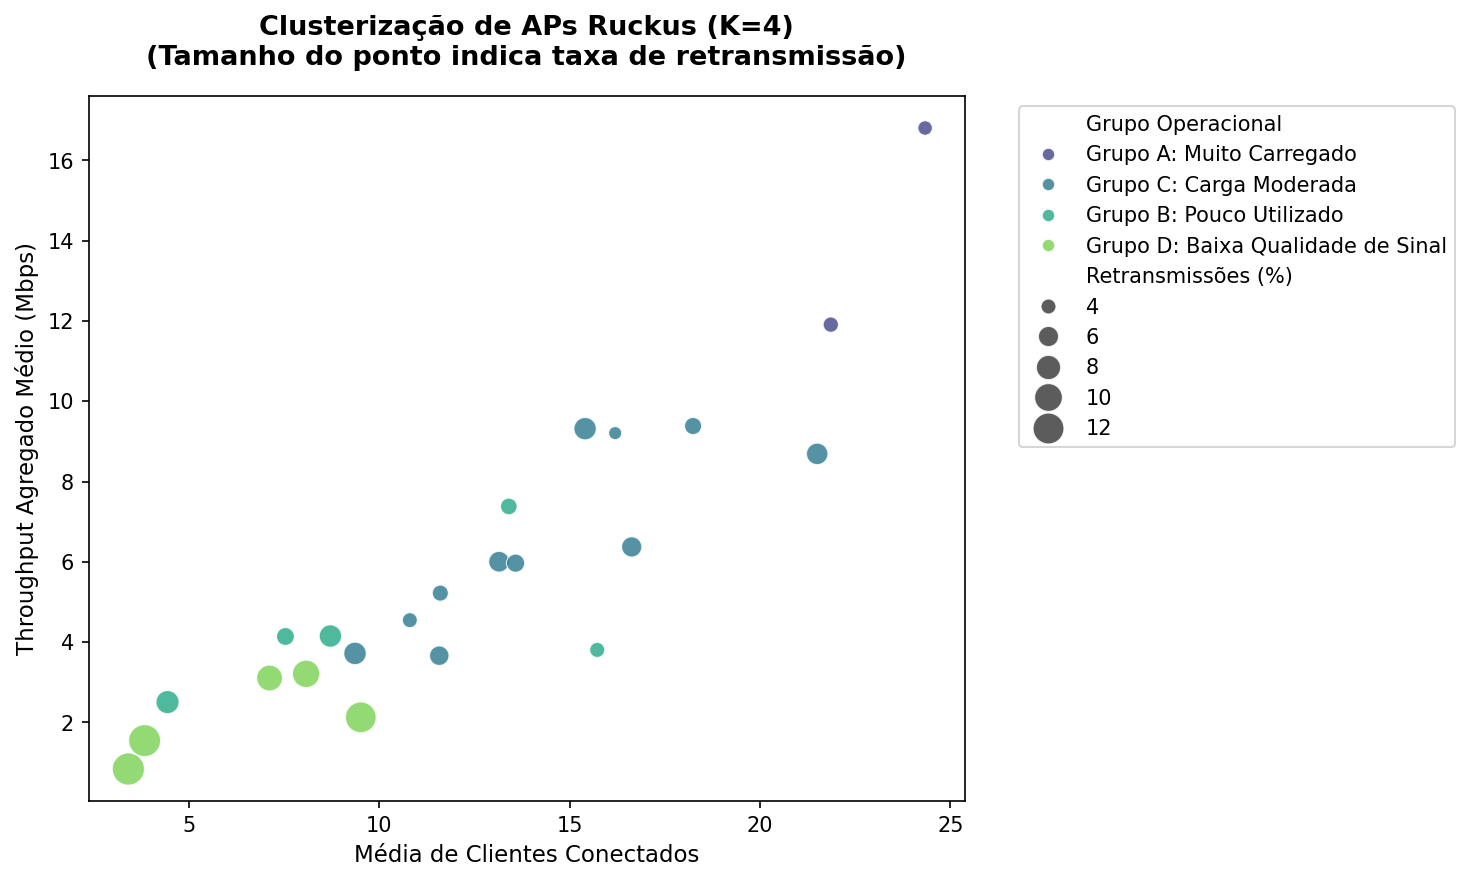
\includegraphics[width=0.85\textwidth]{img/cluster_ruckus.png}
  \caption{Clusterização Ruckus}
  \label{fig:cluster_ruckus_png}
\end{figure}

\begin{itemize}
  \item \textbf{UniFi}:
\end{itemize}
\begin{figure}[H]
  \centering
  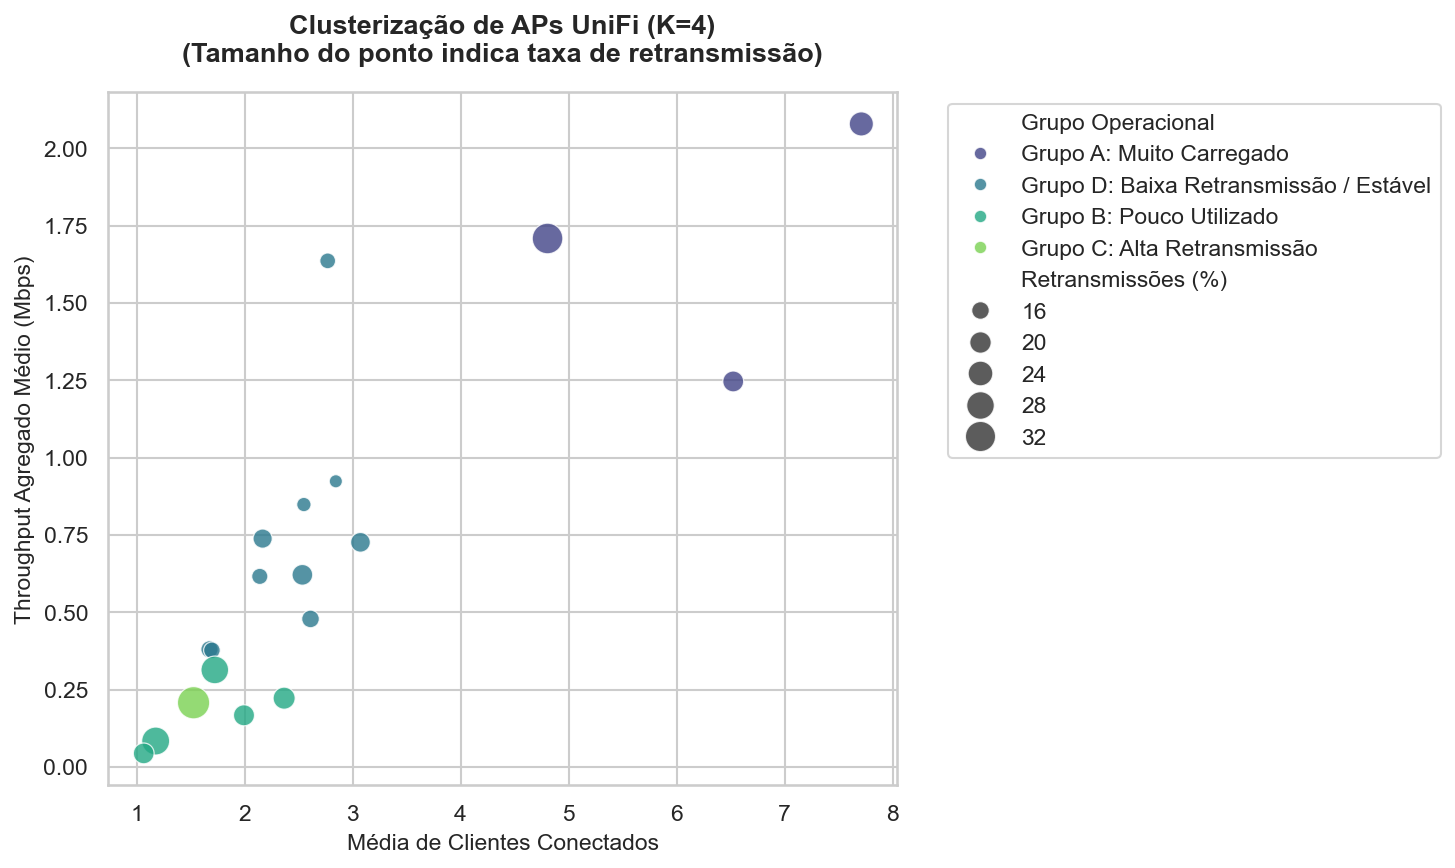
\includegraphics[width=0.85\textwidth]{img/cluster_unifi.png}
  \caption{Clusterização UniFi}
  \label{fig:cluster_unifi_png}
\end{figure}


